
\section{Results}\label{sec:results}
\subsection{Abundance Distribution}
In Figure~\ref{fig:fig1}, briefly discussed in the Introduction, we show the abundance distribution of the Milky Way as well as two of our idealized merger simulations. A number of our idealized simulations exhibit either a bimodal or unimodal abundance distribution, and so we have selected two which are representative examples of 

\begin{figure*}
  \centering
  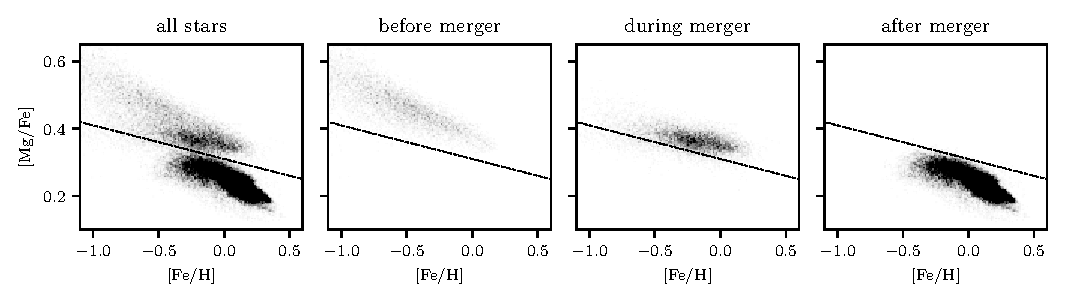
\includegraphics[width=\textwidth]{before_after.pdf}
  \caption{\textbf{The high-$\alpha$ sequence forms before the merger, the low-$\alpha$ sequence forms after the merger.} This plot shows the sequence of events leading to the build-up of the low- and high-$\alpha$ sequences for our fiducial bimodal simulation. We have separated the high- and low-$\alpha$ sequences by a dashed line at $-0.1\FeH + 0.31$, which was chosen by eye to lie in the trough. The left panel shows all star particles in our solar neighborhood cut. The middle left panel shows the star particles that form before the merger ($\tform < 1.5\,\Gyr$), which form a weak sequence of star particles at the lowest \FeH and highest \MgFe. The middle right panel shows the star particles that form during the merger ($1.5\,\Gyr < \tform < 2.5\,\Gyr$). These star particless form the portion of the high-$\alpha$ sequence closest to the trough, and the density of star particless is higher than those that form before. The middle right panel shows the star particles which form after the merger ($\tform > 2.5\,\Gyr$). These star particles form almost entirely below the trough.}
  \label{fig:before_after}
\end{figure*}

\begin{figure}
  \centering
  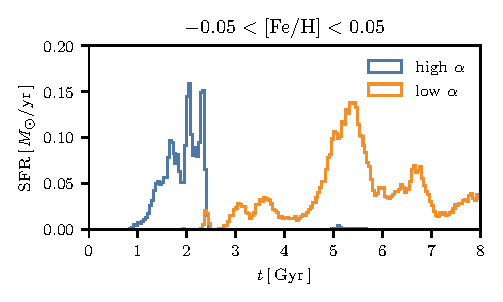
\includegraphics[width=\columnwidth]{before_after_sfh.pdf}
  \caption{\textbf{At fixed metallicity, the low- and high-$\alpha$ sequence are cleanly separated in time, with an intervening quiescent period.} Here we show the star formation history of the high- and low-$\alpha$ sequences. The blue (low-$\alpha$) and orange (high-$\alpha$) histograms correspond to the dashed line cut made in the \MgFe-\FeH plane in Figure~\ref{fig:before_after}, at a fixed metallicity of $\FeH\sim0$. One can see that there is a nearly perfect separation in time between the formation of the high-$\alpha$ and low-$\alpha$ sequence, except for a brief overlap which can be attributed to the inadequacy of the linear cut model of the two sequences. Separating the formation periods lies a quiescent period with a duration of $\sim300\,\Myr$. \red{make sfr per dex}.}
  \label{fig:before_after_sfh}
\end{figure}

\begin{figure}
  \centering
  \includegraphics[width=\columnwidth]{before_after_sfh_by_iron.pdf}
  \caption{\textbf{The timing of the quiescent period which divides the high- and low-$\alpha$ sequences is metallicity dependent.} The star formation history of stars at various fixed metallicities ($\FeH\sim0$, $-0.25$, and $-0.5\,\textrm{dex}$). As in Figure~\ref{fig:before_after_sfh}, there is a quiescent period period which separates the formation of the low- and high-$\alpha$ sequence \red{maybe a better way to show this?}. However, one can see that the timing of the quiescent period is metallicity-dependent. It occurs earlier at lower metallicity, by $\sim300\,\Myr$ for the metallicities shown in this plot. \red{make sfr per dex}.}
  \label{fig:before_after_sfh_by_iron}
\end{figure}

\begin{figure*}
  \centering
  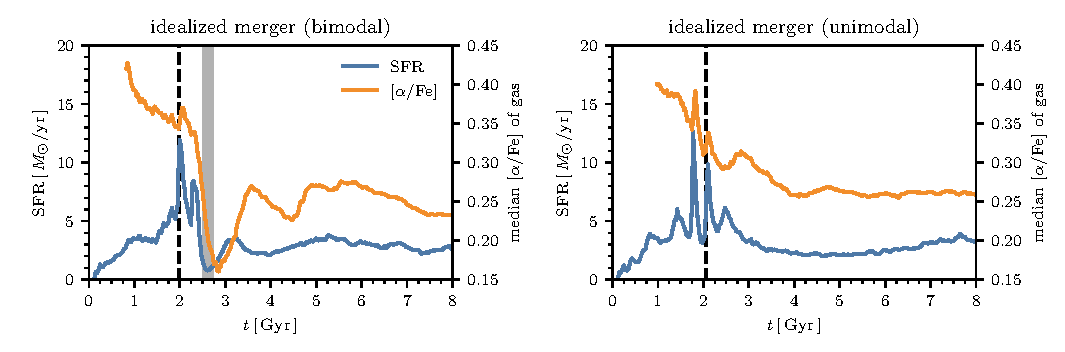
\includegraphics[width=\textwidth]{SFR_alpha.pdf}
  \caption{\textbf{A global suppression of star formation is associcated with a decrease in \MgFe{}, which is seen in the bimodal simulation but not in the unimodal simulation.} Here, we show both the SFR of the central galaxy ($r<15\,\kpc$) and the median \MgFe{} for gas at $2\,\kpc<r<5\,\kpc$ at a fixed \FeH{} bin centered on $-0.2$ with width $0.02\,\dex$. The left panel shows the bimodal simulation while the right panel shows the unimodal simulation. The time of the merger (i.e., the second pericenter) is indicated by the vertical dashed line. In the bimodal simulation, the star formation is suppressed after the merger. This suppression of star formation is associated with a sudden drop in the median \MgFe{} of the gas. Neither the suppression of star formation nor the drop in \MgFe{} are seen in the unimodal simulation.}
  \label{fig:SFR_alpha}
\end{figure*}
